\documentclass[final]{beamer}
\usepackage[size=a0,orientation=portrait,scale=1.0]{beamerposter}
\usepackage{graphicx}
\usepackage{lmodern} % for better fonts
\usepackage{tikz}
\usepackage{multicol}
\usepackage{wrapfig}

% Color scheme
\definecolor{maincolor}{RGB}{0, 70, 140}  % Deep blue
\definecolor{lightgray}{RGB}{240,240,240}

% Poster settings
\title{Hacking on the Software Stack at VSC}
\author{Adam McCartney, Luis Casillas-Trujillo, Filip Kocina, Moritz Siegel,
Atul Singh
\quad | \quad VSC Research Center}
\date{\today}

\setbeamercolor{block title}{fg=white,bg=maincolor}
\setbeamercolor{block body}{fg=black,bg=white}
\setbeamercolor{background canvas}{bg=lightgray}

% Increase block title size
\setbeamerfont{block title}{size=\LARGE,series=\bfseries}
\setbeamerfont{block body}{size=\normalsize}

%%%%%%%%%%%%%%%%%%%%%%%%%%
% code snippet setup
%%%%%%%%%%%%%%%%%%%%%%%%%%
\usepackage{listings}
\usepackage{xcolor}

\lstset{
  basicstyle=\ttfamily\small,
  backgroundcolor=\color{white},
  frame=single,
  rulecolor=\color{gray},
  keywordstyle=\color{blue},
  commentstyle=\color{gray},
  stringstyle=\color{orange},
  breaklines=true,
  showstringspaces=false,
  tabsize=2,
  captionpos=b
}


\begin{document}
\begin{frame}[t]

% Title
\begin{center}
  \vspace{1cm}
  \usebeamercolor[fg]{title}
  \Huge \textbf{\inserttitle}
  
  \vspace{0.5cm}
  \Large \insertauthor
  
  \vspace{1cm}
\end{center}


%%%%%%%%%%%%
%% Variables
%%%%%%%%%%%%

\def\vsc{\textit{VSC}}
\def\sam{\textit{Software and Modules}}
\def\platform{\textit{Platform}}
\def\musica{\textit{MUSICA}}
\def\support{\textit{Support}}
\def\sysadmin{\textit{Sysadmin}}

\def\cern{\textit{CERN}}
\def\cvmfs{\textit{CVMFS}}
\def\easybuild{\textit{EasyBuild}}
\def\eessi{\textit{EESSI}}
\def\gentoo{\textit{gentoo}}
\def\guix{\textit{guix}}
\def\lmod{\textit{Lmod}}
\def\nix{\textit{nix}}
\def\reframe{\textit{ReFrame}}
\def\spack{\textit{Spack}}
\def\sse{\textit{sse2}}

%%%%%%%%%%%%%%%%%%%%%%%%%%%%%%%%%
% Begin content
%%%%%%%%%%%%%%%%%%%%%%%%%%%%%%%%%
\begin{columns}[t]
  \begin{column}{0.48\textwidth}

    \begin{block}{Introduction}
        \begin{itemize}
          \item The \sam{} working group at \vsc{}, has been working on a new
              software stack with the aim of:
          \begin{itemize}
             \item Improving reproducibility and redeployment.
             \item Establishing clear release cycles.
             \item Creating a more organized and user-friendly representation for the cluster users.
          \end{itemize} 


          \item The legacy software stack at \vsc{} evolved from manual
          installation to using \spack{}, which improved dependency
          management, but also introduced issues such as performance
          degradation, global module namespace pollution, and lack of a
          compatibility layer or update mechanism.

          \item The existing GPFS-based file system was found suboptimal
          for software distribution. \cvmfs{} was identified as a more
          scalable solution for distributing metadata-heavy scientific
          software using HTTP and layered web caching.

          \item Inspired by Compute Canada and \eessi{}, the new stack design
              layers \cvmfs{} with a lightweight compatibility layer (based on
                \gentoo{} Prefix) to ensure portability across operating systems and enable consistent builds.

          \item \lmod{} was chosen for organizing software modules into
          structured collections (profiles), and \eessi{}'s extendable
          structure was leveraged to support user, site-wide, and
          project-specific installations via \easybuild{}.
        \end{itemize}
    \end{block}

    \begin{block}{Evolution}
     \begin{itemize}
      \item The evolution of the software stack followed key stages:
      \begin{itemize}
        \item \vsc{} \textbf{1–2}: Software installed manually by expert users.
        \item \vsc{} \textbf{3–4}: Managed by custom scripts; more structure introduced.
        \item \vsc{} \textbf{4–5}: Adoption of \spack{} allowed faster installation and automatic dependency handling.
      \end{itemize}
      \item Challenges
      \begin{itemize}
        \item Complex software presentation.
        \item Unresolved issues around de-duplication.
        \item Organizational strain during OS upgrades with little test coverage.
        \item \musica{} introduces the need to distribute software across sites.
      \end{itemize}
     \end{itemize}
    \end{block}
    \vfill

    \begin{block}{Methods}
        \begin{itemize}
            \item In 2024, the \sam{} working group starts to explore solutions.
            \item October - December 2024, evaluation of: \spack{}, \guix{}, \nix{}, \easybuild{}, \eessi{}, \lmod{}, and \reframe{}
          \item Early 2025, two contrasting strategies were implemented on \musica{}
          \begin{itemize}
              \item \eessi{} \textbf{on the side}: Host-based installs using
                  \easybuild{} and the \sse{} toolkit, with limited \eessi{} integration.
              \item \eessi{} \textbf{as a base}: All software builds will be
                  integrated into \eessi{}'s compatibility layer.
                \begin{itemize}
                  \item \texttt{EESSI\_USER\_INSTALL}
                  \item \texttt{EESSI\_SITE\_INSTALL}
                  \item \texttt{EESSI\_PROJECT\_INSTALL} to \texttt{/cvmfs/software.asc.ac.at}
                \end{itemize}
          \end{itemize}
          \item Test stack: AOCC, Intel compilers, NVHPC, VASP 6.5.0 (CPU \& GPU), Mathematica, Containers.

        \end{itemize}
    \end{block}
    \vfill

    \begin{block}{Distribution across sites with CVMFS}
      \begin{center}
        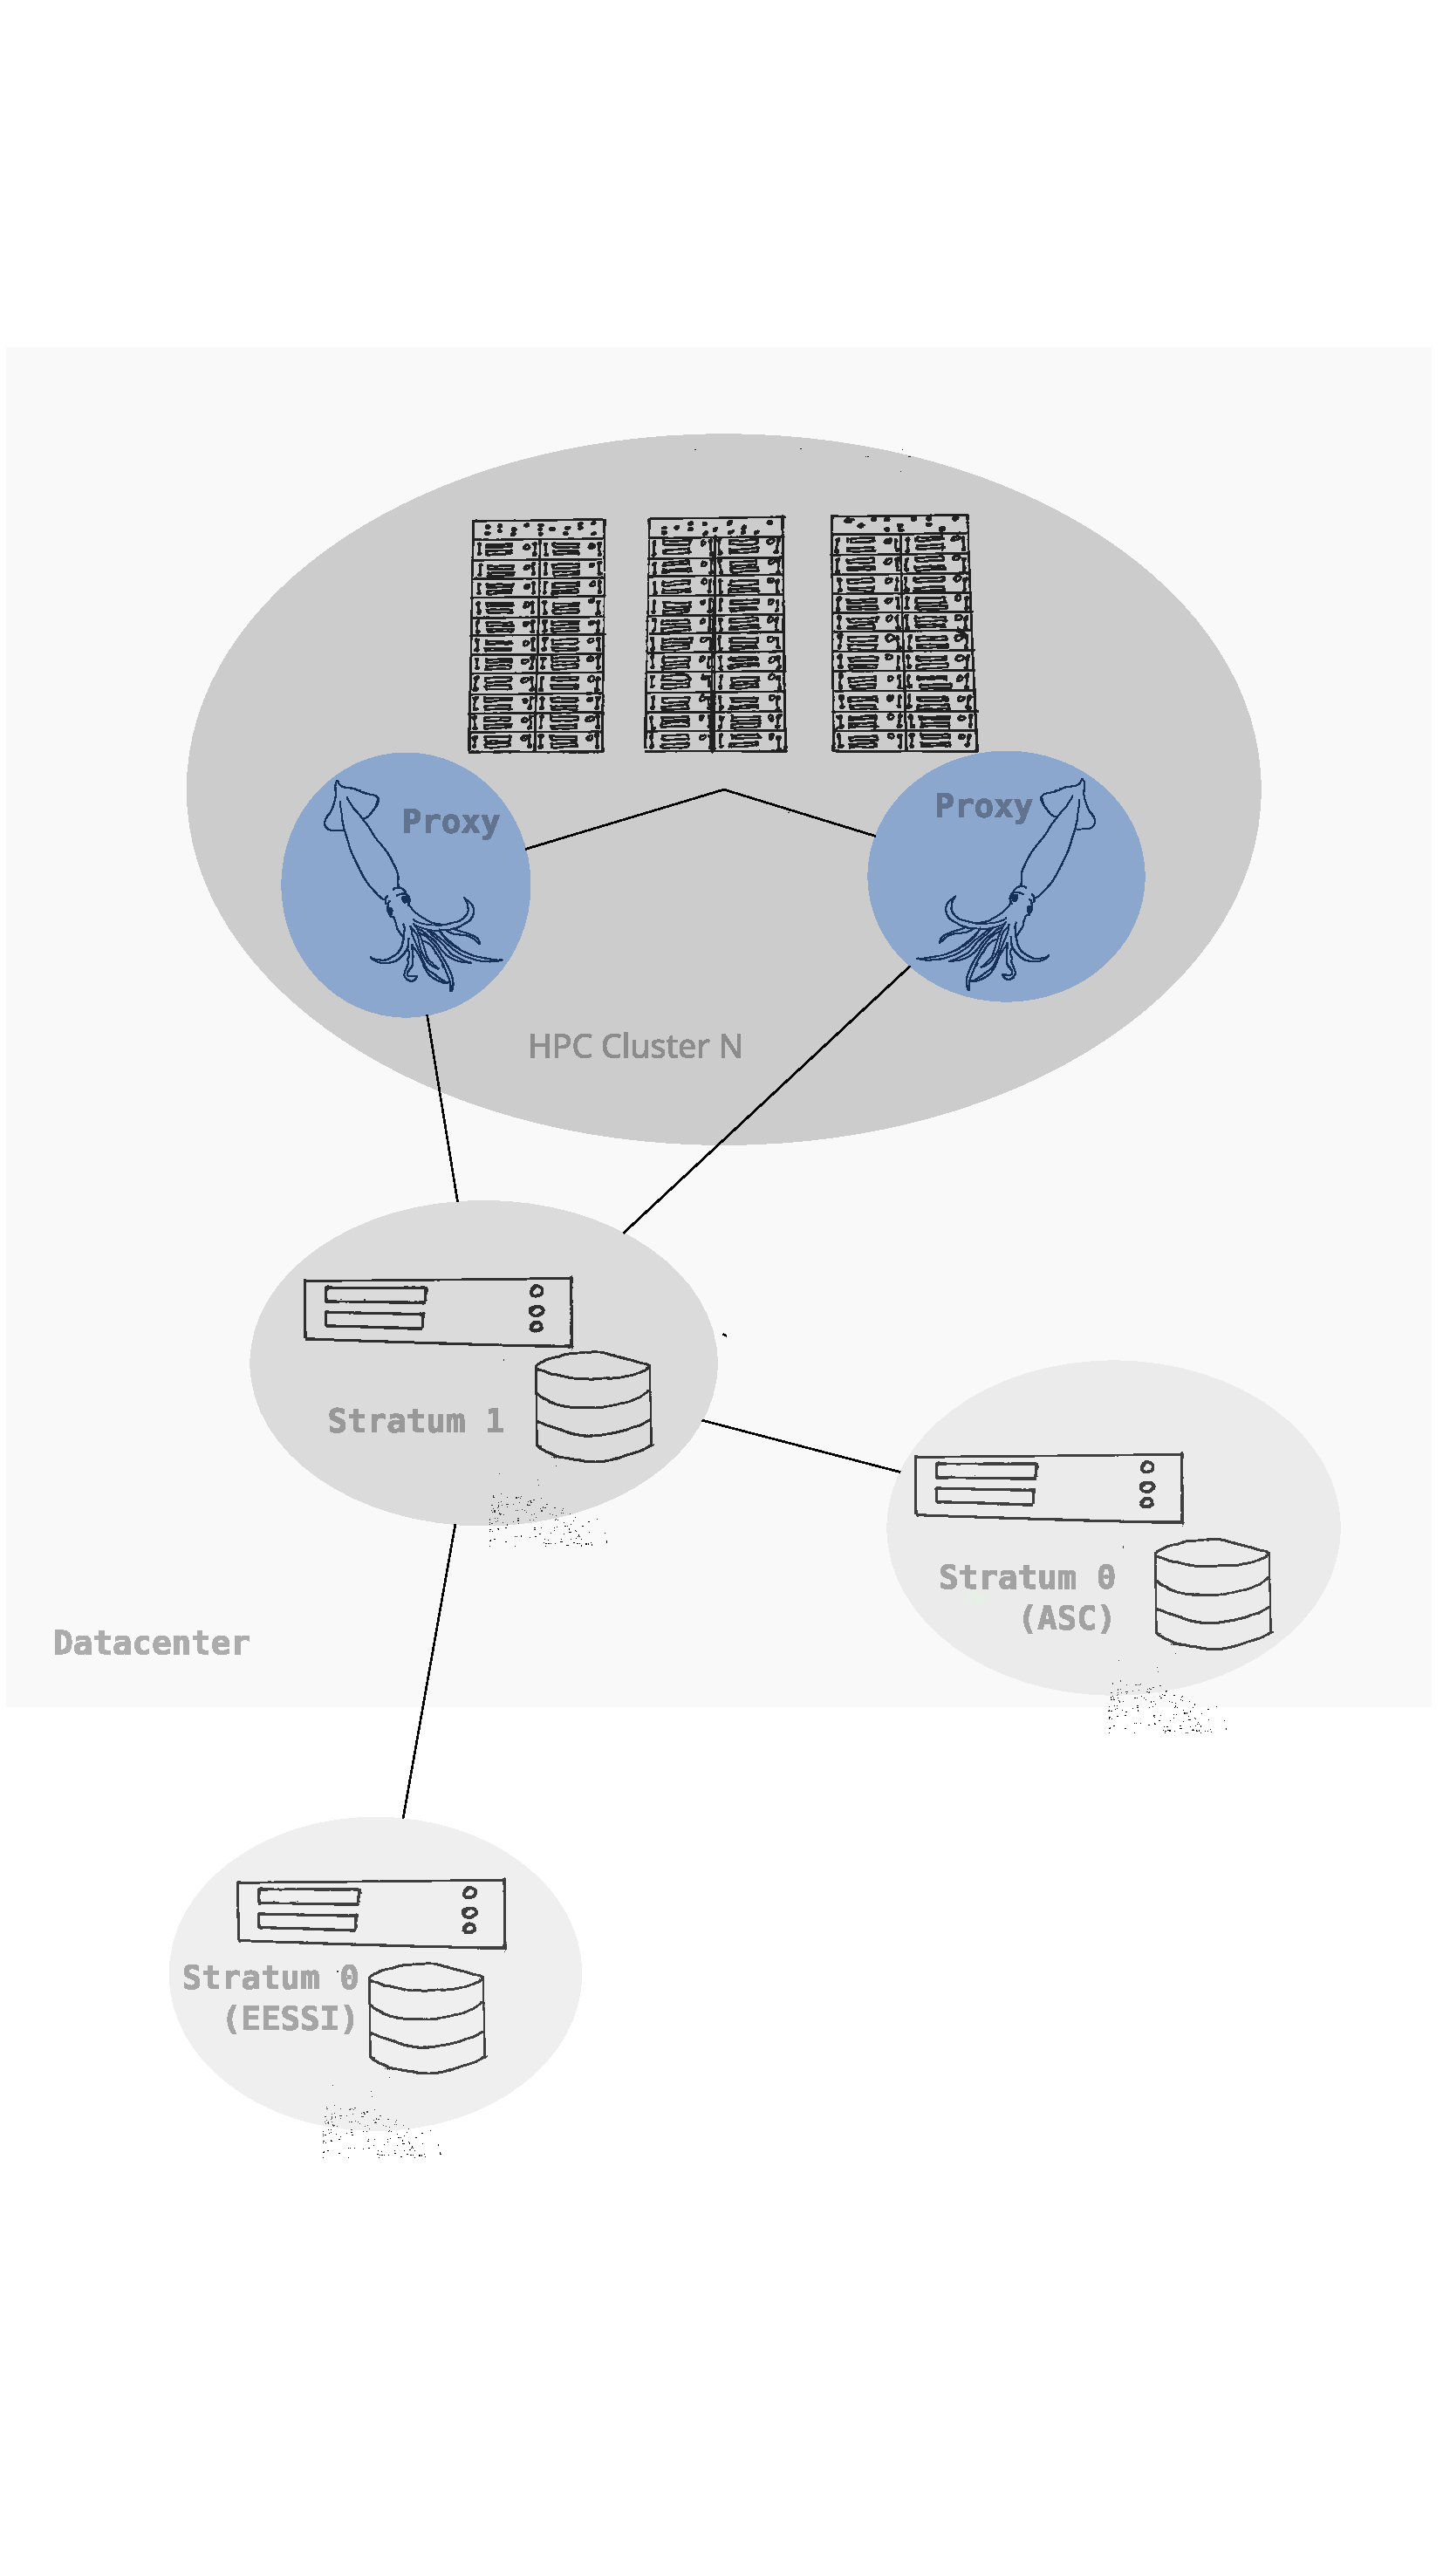
\includegraphics[width=0.75\textwidth]{./include/main_cvmfs.pdf}
      \end{center}
    \end{block}
  \end{column}



  \begin{column}{0.48\textwidth}

      \begin{block}{Compatibility Layer}
          \begin{itemize}
           \item Defined and shipped by \eessi{} as part of a versioned release
           \item The compatibility layer defines a Linux file system hierarchy,
               includes things like libc, basic compilers and interpreters.
           \item Ensures isolation from the host.
          \end{itemize}
      \end{block}

      \begin{block}{Software Layer}
          \begin{itemize}
              \item Software and dependencies can be loaded via environment modules.
              \item System architecture is automatically identified with
                  arch detect.
              \item All software distributed by \eessi{} links against the
                  compatibility layer, so does any software built with
                  EESSI-extend.
          \end{itemize}
      \end{block}


      \begin{block}{EESSI-extend}
          \begin{itemize}
              \item Loads a module containing an \easybuild{} configuration.
              \item Install location is specified through environment variables.
           \end{itemize}
      \end{block}
      
      \begin{block}{Build time}
        \lstinputlisting[language=bash]{./include/snippet-1.bash}
      \end{block}

      \begin{block}{Run time}
        \lstinputlisting[language=bash]{./include/snippet-2.bash}
      \end{block}




      \begin{block} {Key challenges and observations}
          \begin{itemize}
              \item Implicit \easybuild{} configuration is always loaded with
                EESSI-extend, it's not initially obvious what is going on in the
                  background. Also the distributed configuration makes certain
                  assumptions that may not suit all sites.
            \item EasyBlocks bundled with \eessi{} may not build cleanly under EESSI-extend.
            \item Cross-location side effects (e.g., user installs affecting site-wide setups) were observed.
            \item There will always be some interface to host (e.g., Mellanox OFED
                libraries) this requires taking care to compile SLURM with
                  dependencies that are compatible with the MPI software
                  delivered with \eessi{}.
          \end{itemize}
      \end{block}

  \end{column}
\end{columns}

\vfill
\begin{block}{\centering \normalsize Tools and Technologies}
  \centering
  
\includegraphics[width=0.66\paperwidth]{./include/logos.pdf}
\end{block}

\end{frame}
\end{document}

